119. \begin{figure}[ht!]
\center{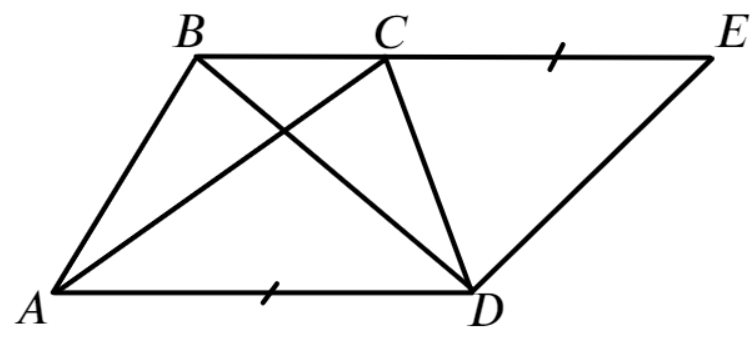
\includegraphics[scale=0.35]{g9-119.png}}
\end{figure}\\
Пусть $BD=4\text{ см},\ AC=3\text{ см}.$ Проведём через точку $D$ прямую, параллельную $AC,$ которая пересечёт продолжение $BC$ в точке $E.$ Тогда $ACED$ является параллелограммом и $DE=AC=3\text{ см},\ CE=AD.$ Средняя линия трапеции равна 2,5 см, значит $AD+BC=2\cdot2,5=5\text{ см}$ и $BE=BC+CE=BC+AD=5\text{ см}.$ Если провести из точки $D$ высоту $DH,$ то $S_{ABCD}=\cfrac{1}{2}\cdot DH\cdot (BC+AD)=\cfrac{1}{2}\cdot DH\cdot BE=S_{\Delta DBE}.$ Треугольник $DBE$ является прямоугольным, так как $BD^2+DE^2=4^2+3^2=5^2=BE^2,$ поэтому $S_{\Delta DBE}=\cfrac{3\cdot4}{2}=6\text{ см}^2.$\\
